\section{ПРОЕКТИРОВАНИЕ ПРОГРАММНОГО КОМПЛЕКСА}

Важным этапом разработки любого программного комплекса является его проектирование. Любой проект, связанный с созданием программного продукта, требует предварительного проектирования, построения структуры и планирования сроков разработки. После предварительного утверждения плана разработки и выбора используемых технологий и структуры программного продукта начинается его реализация.

В данном разеделе будет произведен анализ основных требований; рассмотрены этапы проектирования основных модулей системы.

\subsection{Анализ требований и постановка задачи}

Разработанный программный прогаммный комплекс по управлению централизованными продажами в системе Bycard должен предоставить единый интерфейс для покупки билетов на мероприятия. Это значительно облегчит разработку клиентов для продажи билетов: мобильных приложений, сайта.

Система должна аггрегировать актуальную информацию о проходящих мероприятиях: расписание, цены на билеты, наличие доступных для продажи мест, возможность покупки билета онлайн. А также предоставить информационными ресурсам удобный механизм интерграции, благодаря которому будет возможность размещать актуальную афишу мероприятий на сторонних сайтах, показывать кнопки для покупки билета.

Большое значение имеют затраты на подключение к системе группы новых объектов, синхронизации данных между ними. Необходимо разработать механизм, который позволит подключать к системе объекты для продажи билетов с минимальными затратами.

\subsection{Основные модули системы}

\subsubsection{API}

Данный модуль системы предоставляет общий интерфейс для общения с объектами, подключёнными к системе. Объекты могут иметь различные интерфейсы обмена данными. Например, система для продажи билетов, установленная в кинотеатре наверняка отличается от той, что установлена в театрах, филармонии, концертных залах и т.д. Поэтому логично будет написать для каждой группы объектов отдельный клиент, который будет необходимый интерфейс методов. Для кинотеатров это будет одна реализация, для театров - другая. Обощённая структура изображена на рисунке ~\ref{fig:api-struct}:

В терминах проекта будем далее называть объект, подключенный к системе вебгейтом, а клиент для работы с ним - вебгейт-клиентом. Каждый клиент для вебгейта должен реализовывать необходимый минимум методов, определенных в интерфейсе WebgateClientInterface. Это методы для для реализации фукнции покупки билета: метод блокировки и разблокировки места, создания и отмены заказа. Метод getOrder используется в чекере, который будет описан дальше. Метод getPerformances нужен для получения списка мероприятий, цен на события, которые проходят в конкретном объекте. Система с заданной периодичностью получает актуальную информацию, обновляет её и сохраняет для дальнейшего использования. Эти и другие методы приведены в листинге ~\ref{lst:wci}

\begin{figure}
  	\centering
 	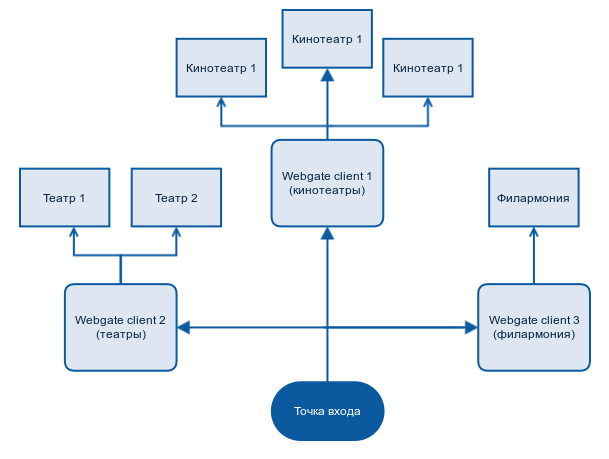
\includegraphics[width=1\textwidth]{images/api-struct.png}
  	\caption{Структура API}
    \label{fig:api-struct}
\end{figure}

\begin{lstlisting}[language=PHP,caption={WebgateCleintInterface}label=lst:wci]
interface WebgateClientInterface
{
	public function getPerformances();
	public function authorize();
	public function lockPlace();
	public function unlockPlace();
	public function createOrder();
	public function cancelOrder();
	public function unlockPlaces();
	public function getPlaces();
	public function addPayment();
	public function returnPlace();
	public function getOrder();
}
\end{lstlisting}




